\documentclass{beamer}
%
% Choose how your presentation looks.
%
% For more themes, color themes and font themes, see:
% http://deic.uab.es/~iblanes/beamer_gallery/index_by_theme.html
%
\mode<presentation>
{
  \usetheme{default}      % or try Darmstadt, Madrid, Warsaw, ...
  \usecolortheme{default} % or try albatross, beaver, crane, ...
  \usefonttheme{default}  % or try serif, structurebold, ...
  \setbeamertemplate{navigation symbols}{}
  \setbeamertemplate{caption}[numbered]
} 

\usepackage[english]{babel}
\usepackage[utf8]{inputenc}
\usepackage[T1]{fontenc}
\usepackage{chemist}
\usepackage[version=4]{mhchem}
\usepackage{fancybox}

\title[Your Short Title]{Projet de département  : Formation de patterns dans les systèmes de réaction-diffusion}
\author{Cyril NEDERVEEN\\
Louise HUREL\\
Audrey GOSSARD\\
Dana ZILBERBERG}
\institute{Ecole des Ponts Paristech}

\begin{document}

\begin{frame}
  \titlepage
\end{frame}

% Uncomment these lines for an automatically generated outline.
%\begin{frame}{Outline}
%  \tableofcontents
%\end{frame}

\section{Introduction}

\begin{frame}{Introduction}

\begin{itemize}
  \item Your introduction goes here!
  \item Use \texttt{itemize} to organize your main points.
\end{itemize}

\vskip 1cm

\begin{block}{Examples}
Some examples of commonly used commands and features are included, to help you get started.
\end{block}

\end{frame}

\section{Some \LaTeX{} Examples}

\subsection{Tables and Figures}

\begin{frame}{Tables and Figures}

\begin{itemize}
\item Use \texttt{tabular} for basic tables --- see Table~\ref{tab:widgets}, for example.
\item You can upload a figure (JPEG, PNG or PDF) using the files menu. 
\item To include it in your document, use the \texttt{includegraphics} command (see the comment below in the source code).
\end{itemize}

% Commands to include a figure:
%\begin{figure}
%\includegraphics[width=\textwidth]{your-figure's-file-name}
%\caption{\label{fig:your-figure}Caption goes here.}
%\end{figure}

\begin{table}
\centering
\begin{tabular}{l|r}
Item & Quantity \\\hline
Widgets & 42 \\
Gadgets & 13
\end{tabular}
\caption{\label{tab:widgets}An example table.}
\end{table}

\end{frame}

\subsection{Mathematics}

\begin{frame}{Readable Mathematics}

Let $X_1, X_2, \ldots, X_n$ be a sequence of independent and identically distributed random variables with $\text{E}[X_i] = \mu$ and $\text{Var}[X_i] = \sigma^2 < \infty$, and let
\[ S_n = \frac{X_1 + X_2 + \cdots + X_n}{n}
      = \frac{1}{n}\sum_{i}^{n} X_i \]
denote their mean. Then as $n$ approaches infinity, the random variables $\sqrt{n}(S_n - \mu)$ converge in distribution to a normal $\mathcal{N}(0, \sigma^2)$.

\end{frame}



\subsection{Modélisation de la morphogenèse par des équations de réaction-diffusion}

\begin{frame}{Modélisation de la morphogenèse par des équations de réaction-diffusion}

\begin{columns}
\column{0.5\textwidth}
\underline{Modèle de Schnakenberg :} \\ \medskip
Réaction des espèces X et Y dans milieu avec A et B
    \begin{center}
    \begin{chemmath}
    \begin{split}
        X & \ce{ <=>[k_{1}][k_{-1}] A} \\
        \ce{B & ->[k_{2}][ ] Y} \\
          \ce{2X + Y & ->[k_{3}] 3X}
    \end{split}
    \end{chemmath}
    \end{center}
\column{0.5\textwidth}
\underline{Equation obtenue :} \\ \medskip
$u$ et $v$ = concentrations X et Y (normalisées) \\
$d$ et $\delta$ = paramètres

\medskip

\fboxsep=3pt
\fboxrule=1.7pt
\def\bordercolor{purple}
\def\backgroundcolor{white}
\cornersize{0.9}
\fcolorbox{\bordercolor}{\backgroundcolor} {$
        \frac{\partial c}{\partial t} = D \Delta c + \delta f(c)
    $}
\smallskip

    avec c = \begin{pmatrix} u \\ v \end{pmatrix},
    D = \begin{pmatrix} 
        1  & 0 \\
        0  & d
          \end{pmatrix}
    et f(c) = \begin{pmatrix} a - u + vu^{2} \\ b-vu^{2} \end{pmatrix}.
\end{columns}

\end{frame}



\begin{frame}{Modélisation de la morphogenèse par des équations de réaction-diffusion}

\textbf{\underline{Résolution sans terme de diffusion}}
\begin{equation}
\frac{\partial c}{\partial t} = \delta f(c)
\end{equation}

Solution d'équilibre : 
\begin{cases} $u_{eq} = a+b$ \\
              $v_{eq} = \frac{b}{(a+b)^{2}}$
\end{cases}
\\ \bigskip
Solution d'équilibre \textbf{stable} $\Longleftrightarrow$ $b-a<(a+b)^{3}$.

\end{frame}

\subsection{Diagramme de Turing}

\begin{frame}{Diagramme de Turing}

\begin{itemize}
    \item \underline{linéarisation:} $z = c - c_{eq}$ \quad $f(c) = J_{f}(c_{eq})z$
    $$
    \Rightarrow \frac{dz}{dt} = D\Delta z + \delta J_{f}(c_{eq})z
    $$
    \item \underline{modes de Fourier:}
    $$
    z(x,t) = \sum\limits_{n=0}^{\infty}s_{n}(t) e_{n}(x) \quad (e_{n}(x) = cos(n \pi x))
    $$
    \item \underline{vecteur propre:} $\Delta e_{n}(x) = -(n\pi)^{2} e_{n}(x)$
    $$\Rightarrow \frac{ds_{n}}{dt} = (-(n\pi)^{2}D + \delta J_{f}(c_{eq}))s_{n} $$
    \item \textbf{CNS mode stable} \\
    \medskip
    \fboxsep=3pt
    \fboxrule=1.7pt
    \def\bordercolor{purple}
    \def\backgroundcolor{white}
    \cornersize{0.9}
    \fcolorbox{\bordercolor}{\backgroundcolor} {$tr(-(n\pi)^{2}D + \delta J_{f}(c_{eq})) < 0$ et $det(-(n\pi)^{2}D + \delta J_{f}(c_{eq})) > 0$}
    
    
\end{itemize}

\end{frame}

\begin{frame}{Diagramme de Turing}
    \underline{Premier affichage du diagramme de Turing:}
    
    \begin{columns}

    \begin{column}{250}
    \begin{figure}
    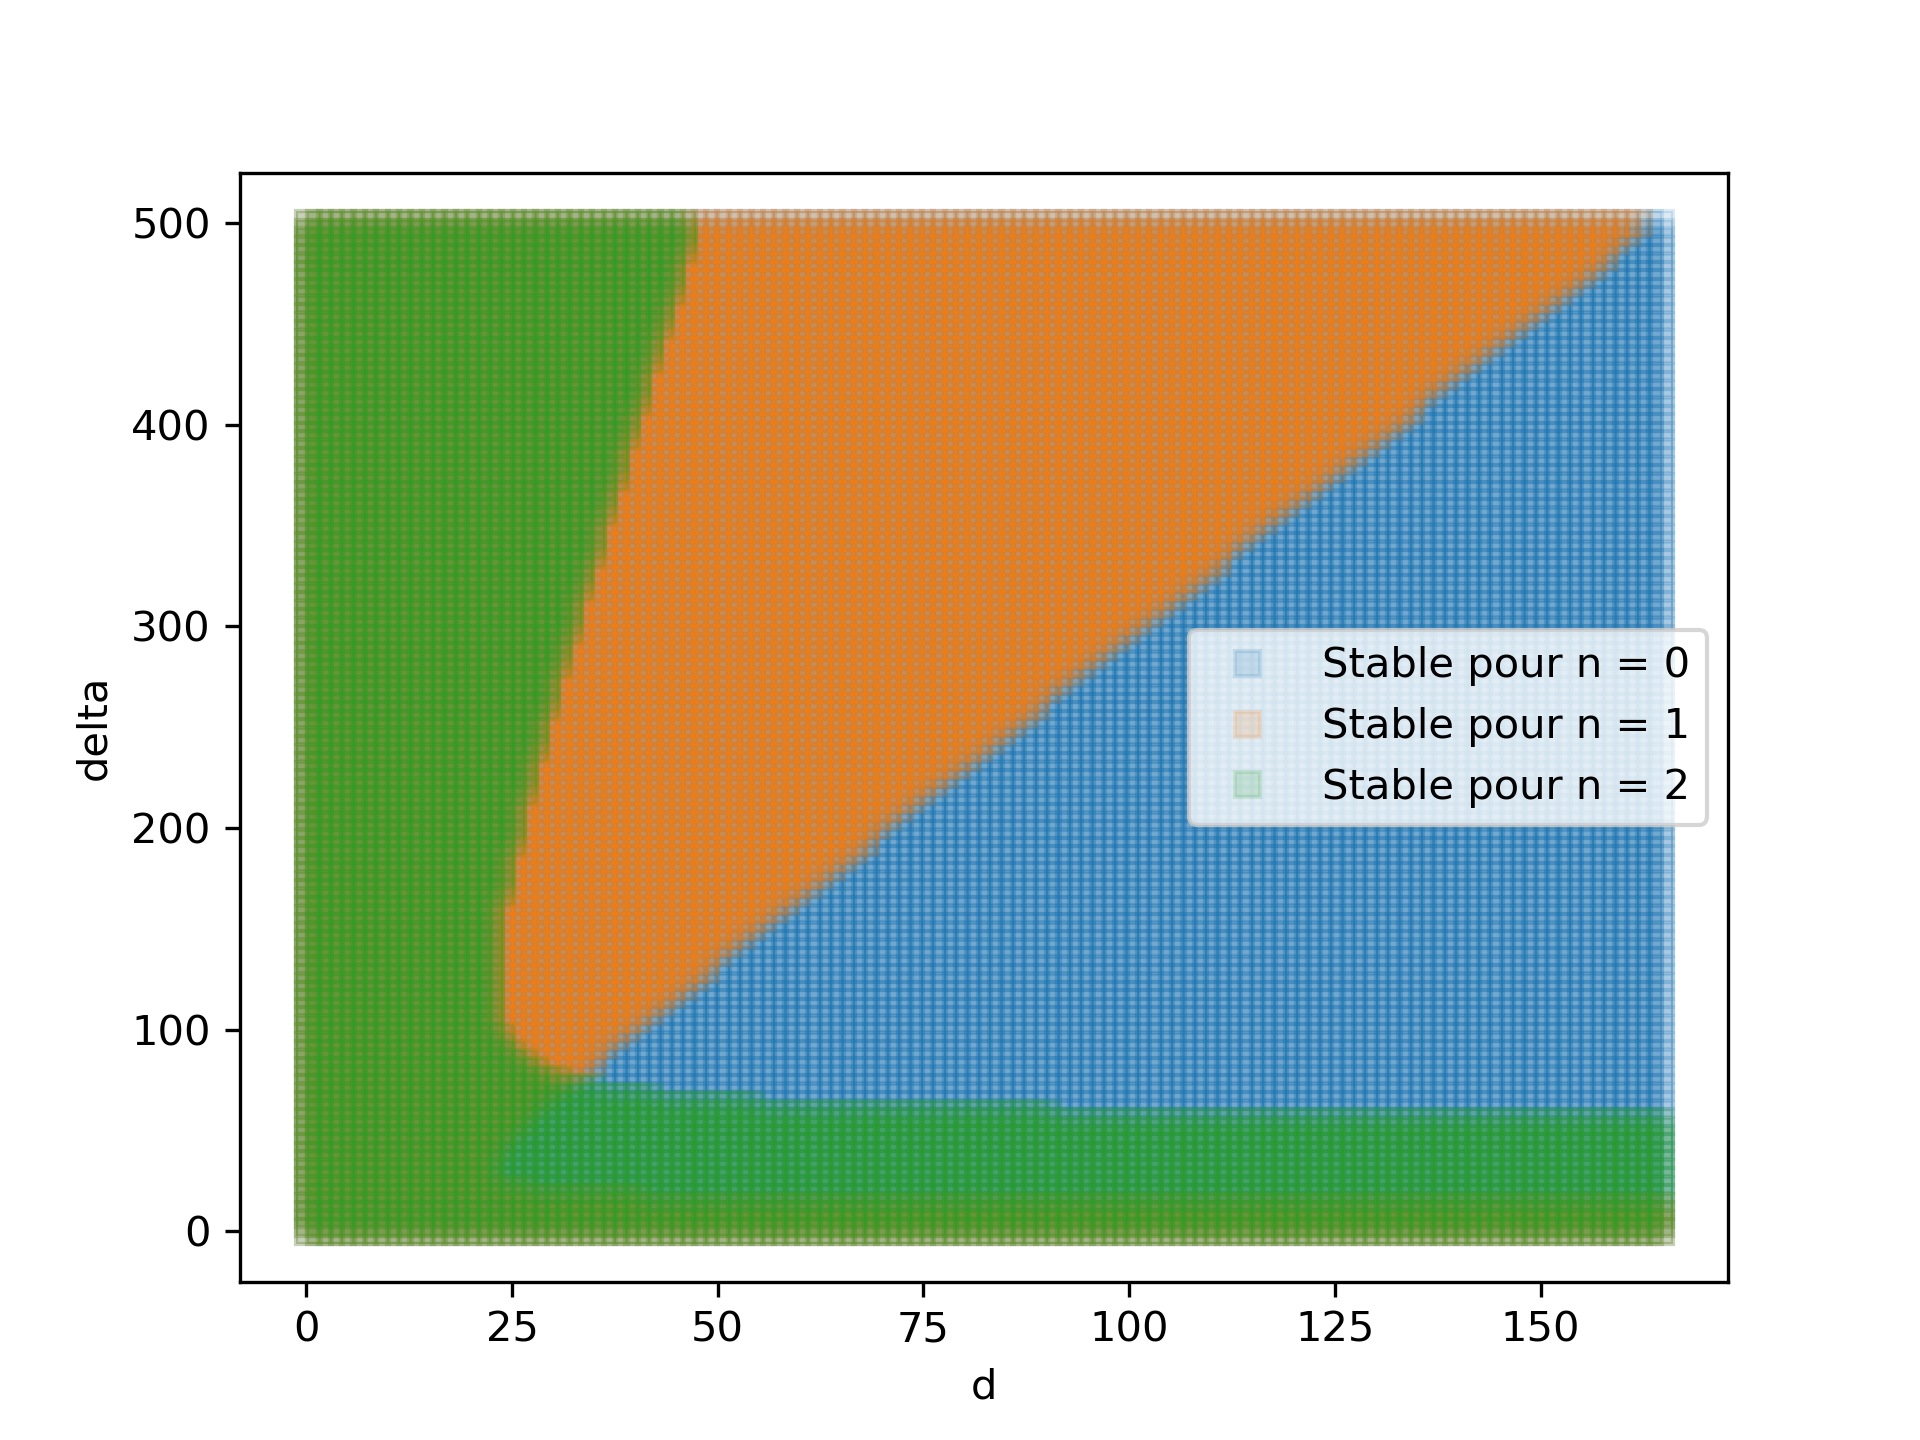
\includegraphics[width=220]{diagrammes_turing3_1.png}
    \caption{\label{diagramme_turing_1}{Diagramme de Turing}}
    \end{figure}
    \end{column}
    
    \begin{column}{2.7cm}
    On parcourt une grille de $\delta$ et $d$, on teste la stabilité de plusieurs modes (ici de 0 à 2). Lorsque la case est colorée, le mode de cette couleur est stable.
    
    \end{column}
    \end{columns}
    
    
\end{frame}

\begin{frame}{Diagramme de Turing}
    \underline{Amélioration de l'affichage du diagramme de Turing:}
    
    \begin{columns}

    \begin{column}{250}
    \begin{figure}
    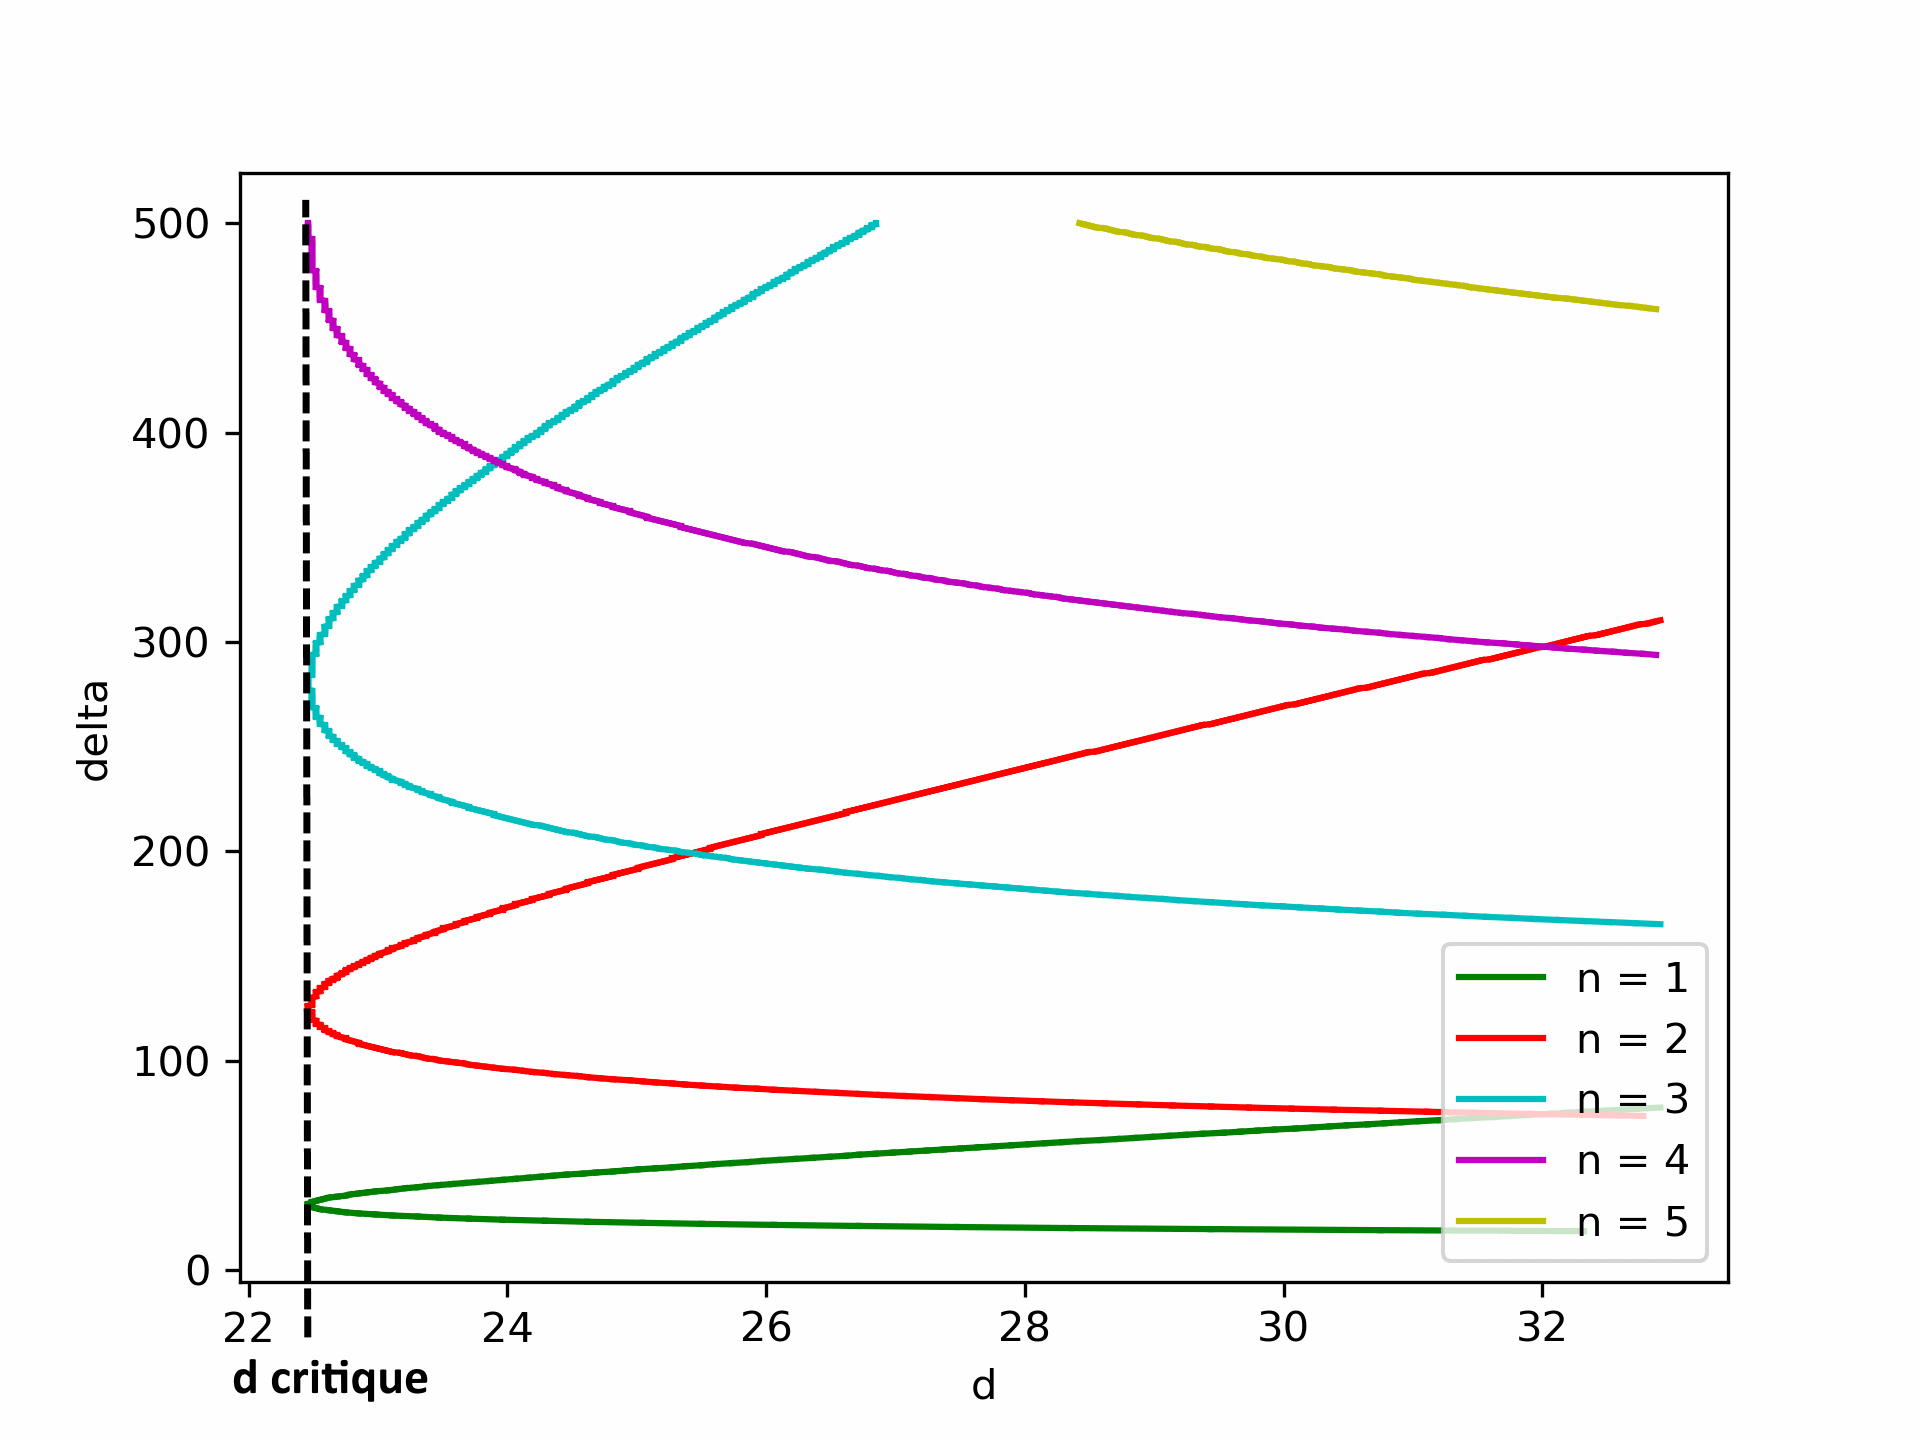
\includegraphics[width=220]{diagrammes_turing_bis_avec_d_crit.png}
    \caption{\label{diagramme_turing_2}{Diagramme de Turing amélioré (modes 1 à 5)}}
    \end{figure}
    \end{column}
    
    \begin{column}{2.7cm}
    On observe un $d_{critique}$ qui semble indépendant de $\delta$ en dessous duquel tous les modes sont stables. \\
    Ligne = frontière de stabilité (gauche stable, droite instable)
    
    \end{column}
    \end{columns}
    
    
\end{frame}




\subsection{Résolution par la méthode d’Euler implicite}

\begin{frame}{Résolution par la méthode d’Euler implicite}
\textbf{Définition des variables et des paramètres :}
\begin{itemize}
    \item $a = 0.2$ et $b = 1.3$ (pour satisfaire $(a+b)^3>b-a$ et $b>a$.\\
    \item $N_x$ le nombre d'it\'erations sur la variable d'espace, $x \in [0;1]$\\
    \item $c = \begin{pmatrix} u \\ v \end{pmatrix}$, de taille $2 N_x$.\\
    \item $dt = 10^{-3}$ et $N_t = 50 000$
    \item variable $stock$ de taille $(2N_x,N_t)$ pour stocker toutes les concentrations
\end{itemize}

\end{frame}

\begin{frame}{Résolution par la méthode d’Euler implicite}
\textbf{Initialisation autour de la solution d'\'equilibre :}
aléatoirement autour de $u_{eq}$ et $v_{eq}$ à $10^{-4}$\\
\begin{figure}
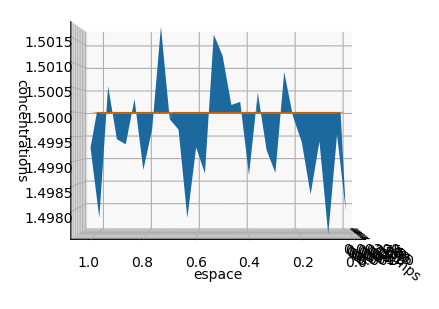
\includegraphics[width=\textwidth]{cond_init.png}
\caption{\label{fig:your-figure}Conditions initiales}
\end{figure}

\end{frame}

\begin{frame}{Résolution par la méthode d’Euler implicite}
\textbf{Equation du schéma}
à l'instant $t_n = n dt$\\
\begin{equation}
c^{n+1} = c^n + dt (DA c^{n+1} + \delta f(c^{n+1}))
\end{equation}
avec D = \begin{pmatrix} 
I  & 0 \\
 0  & dI
\end{pmatrix} et A = \begin{pmatrix} 
Lp  & 0 \\
 0  & Lp
\end{pmatrix}\\ où
\begin{displaymath}
Lp = \frac{1}{dx^2} \begin{pmatrix} 
-2     & 1     & 0      & \cdots & 1\\
 1     & -2    & \ddots & \ddots & \vdots\\
 0     &\ddots & \ddots & \ddots & 0\\
\vdots & \ddots& \ddots & \ddots & 1\\
1      &\cdots & 0      &    1   & -2
\end{pmatrix}
\end{displaymath}

\end{frame}

\begin{frame}{Résolution par la méthode d’Euler implicite}
\textbf{Simplification du schéma :}
\begin{align}
c^{n+1} = c^n + dt (DA c^{n+1} + \delta f(c^n)) \nonumber\\
\nonumber \\
c^{n+1} = (I - dt DA)^{-1} (c^n + dt \delta f(c^n))
\end{align}\\
\textbf{Stockage :}
\begin{equation}
stock(n, 1:2 N_x) = c^n
\end{equation}\\
\end{frame}

\begin{frame}{Résolution par la méthode d’Euler implicite}
\textbf{Résultats}\\
Prévision : instabilité du mode 2, vérifiée
\begin{figure}
\begin{subfigure}
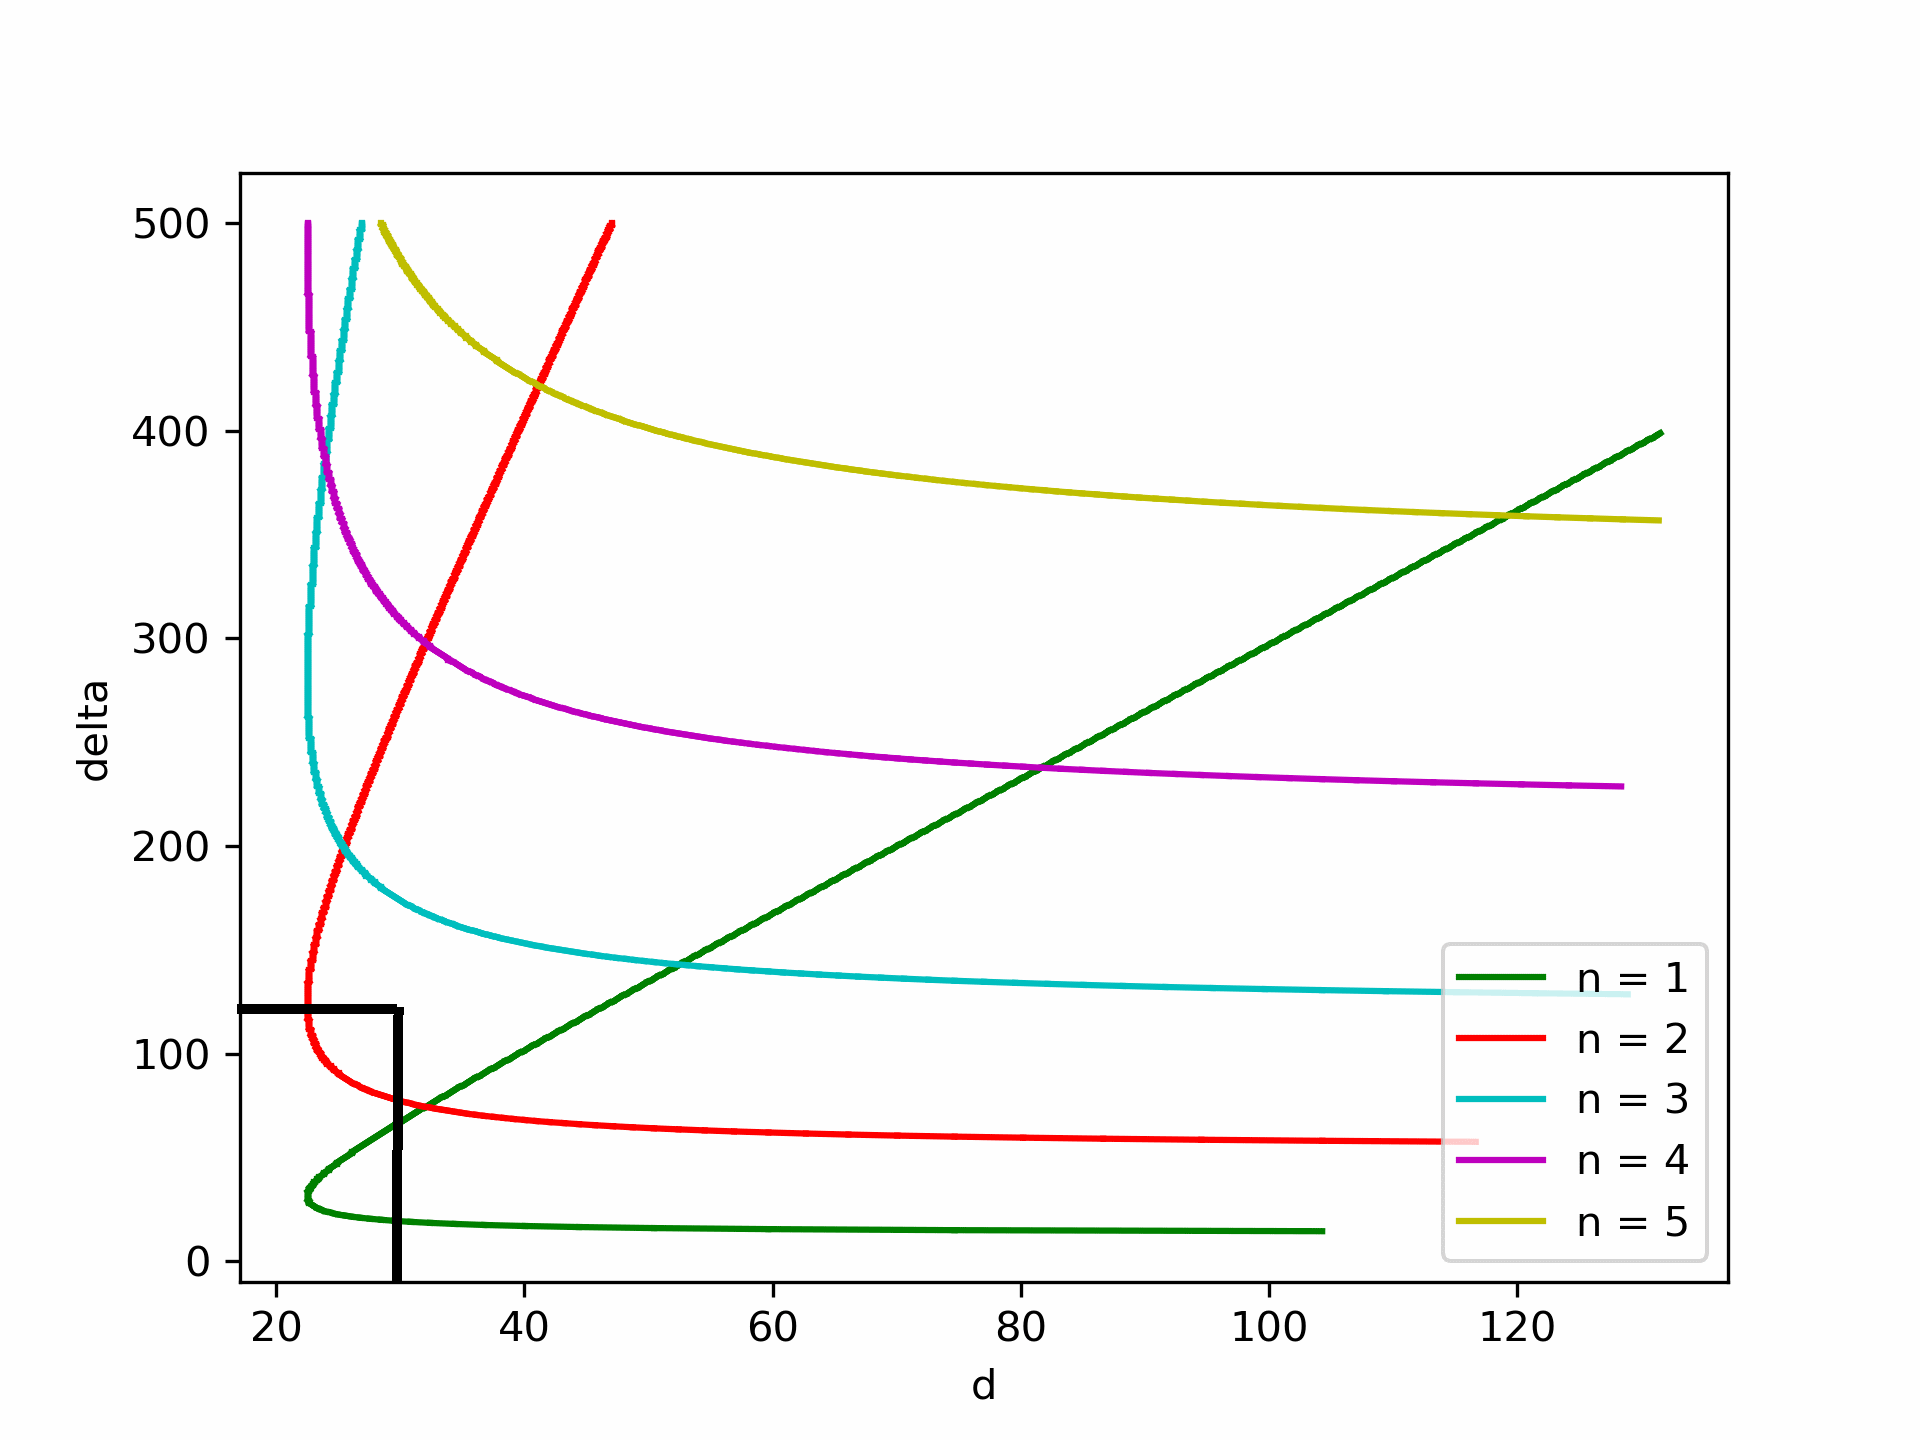
\includegraphics[width=0.4\textwidth]{diagrammes_turing1.png}
\end{subfigure}
\begin{subfigure}
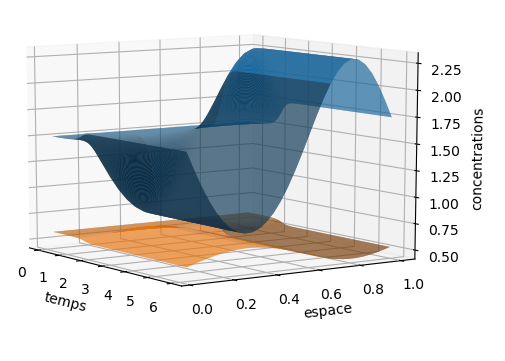
\includegraphics[width=0.4\textwidth]{graph1.png}
\end{subfigure}
\caption{\label{fig:graph1}Instabilité du mode 2}
\end{figure}
\end{frame}


\begin{frame}{Résolution par la méthode d’Euler implicite}
\textbf{Résultats}\\
Prévision : instabilité du mode 4, vérifiée
\begin{figure}
\begin{subfigure}
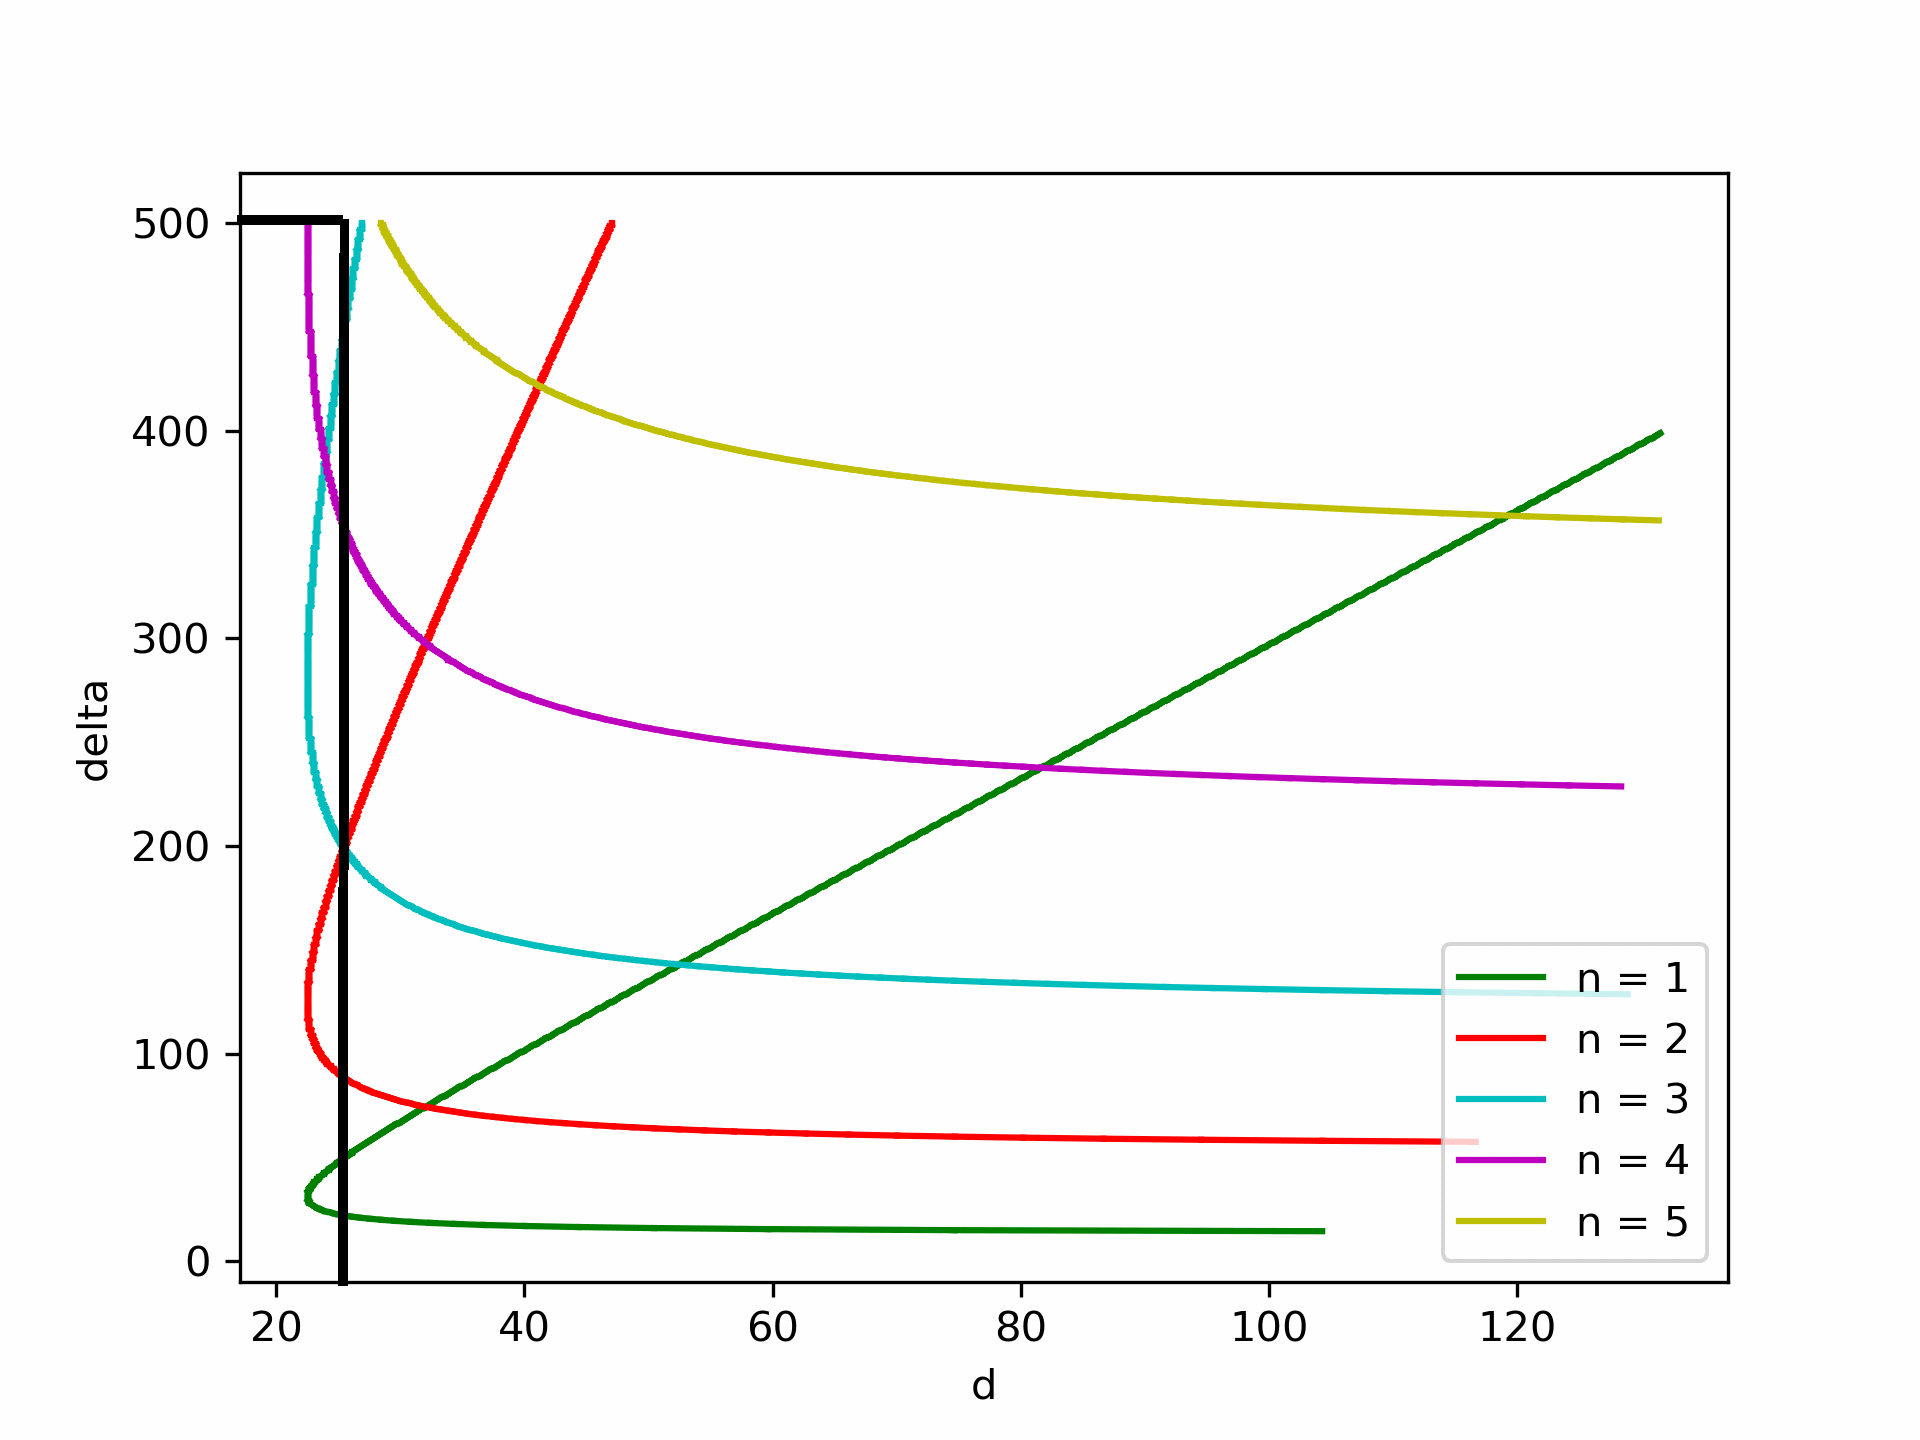
\includegraphics[width=0.4\textwidth]{diagrammes_turing2.png}
\end{subfigure}
\begin{subfigure}
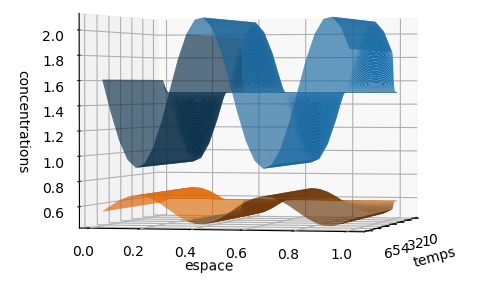
\includegraphics[width=0.4\textwidth]{graph2.png}
\end{subfigure}
\caption{\label{fig:graph1}Instabilité du mode 4}
\end{figure}
\end{frame}

\begin{frame}{Résolution par la méthode d’Euler implicite}
\textbf{Remarques}\\
Superposition de modes instables
\begin{figure}
\begin{subfigure}
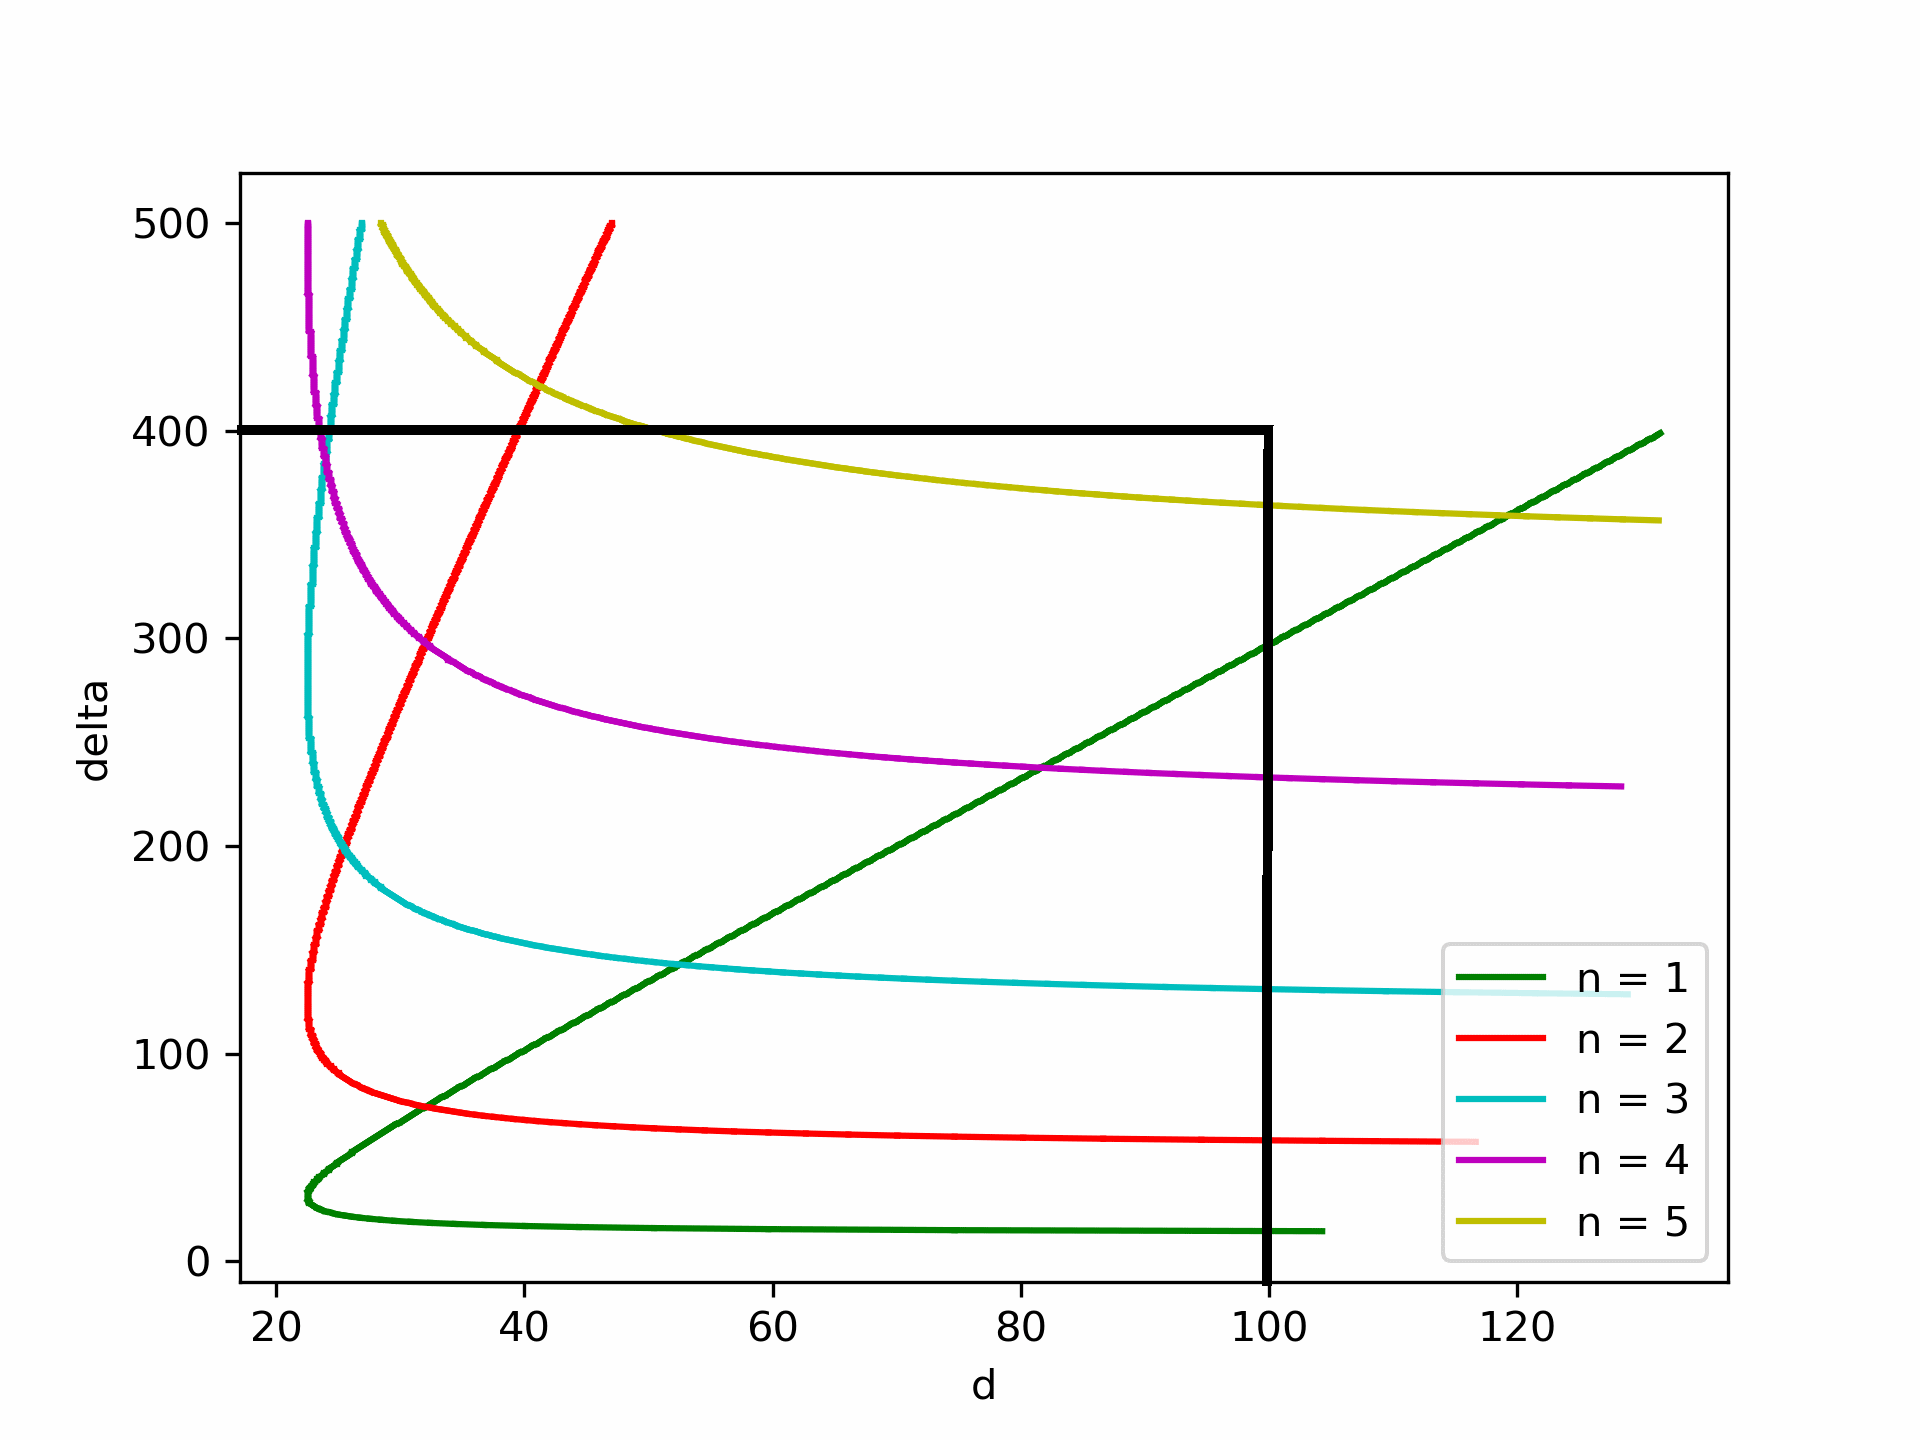
\includegraphics[width=0.4\textwidth]{diagrammes_turing3.png}
\end{subfigure}
\begin{subfigure}
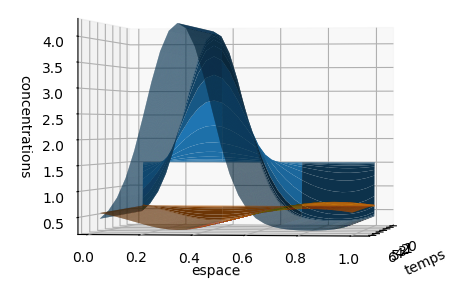
\includegraphics[width=0.4\textwidth]{graph3.png}
\end{subfigure}
\caption{\label{fig:graph3}Superposition des modes instables}
\end{figure}
\end{frame}


\begin{frame}{Résolution par la méthode d’Euler implicite}
\textbf{Remarques}\\
Plus on est proche de $d_{critique}$, plus la convergence apparaît tardivement : 
\begin{figure}
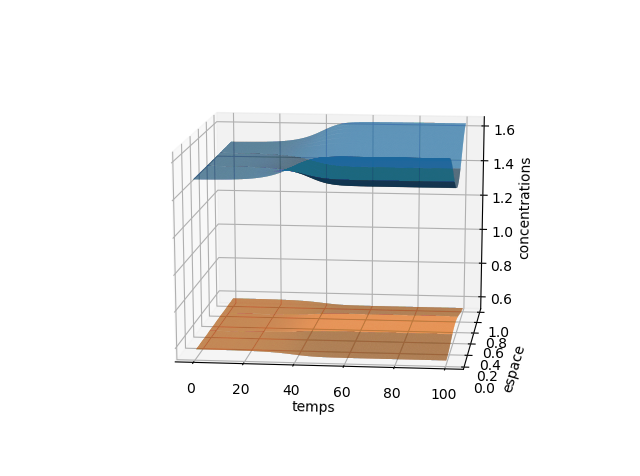
\includegraphics[width=0.4\textwidth]{graph4.png}
\caption{\label{fig:graph4} $d = 23.1$, convergence après 50 secondes}
\end{figure}
\end{frame}



\begin{frame}{Diagramme de Turing expérimental}
Diagramme de Turing expérimental tracé grâce à méthode de résolution:
\begin{itemize}
    \item conditions initiales perturbées (proche de l'équilibre)
    \item stabilisation pendant grand temps
    \item comparaison avec solution d'équilibre -> stabilité ou non
\end{itemize}
\begin{figure}
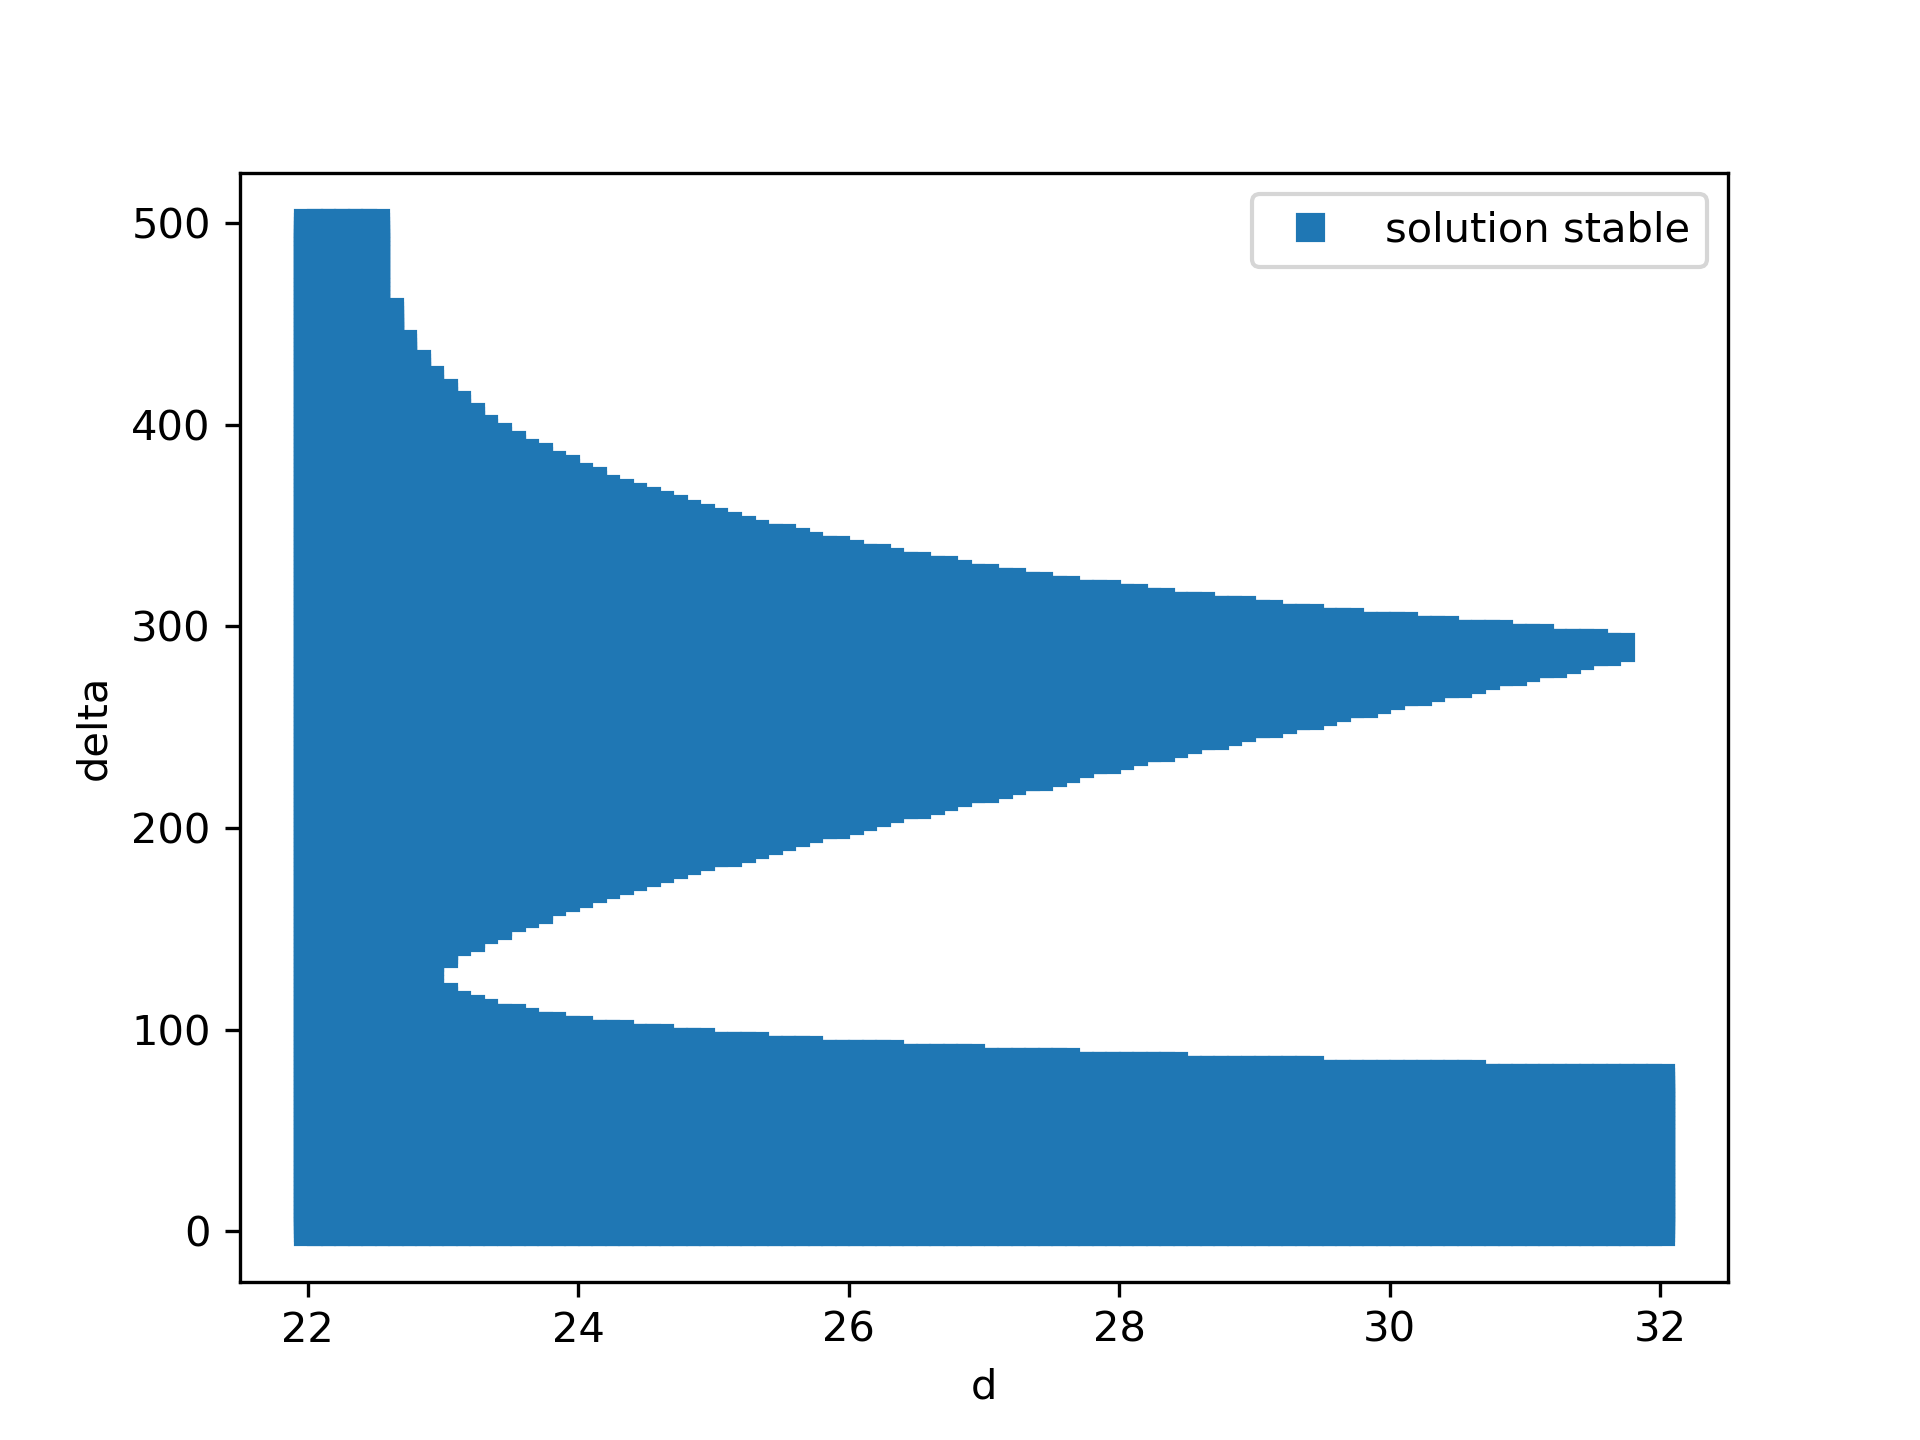
\includegraphics[width=0.45\textwidth]{diagrammes_turing_exp4.png}
\caption{En bleu: solution stable}
\end{figure}
\end{frame}


\begin{frame}{Comparaison des deux diagrammes}
On superpose le diagramme précédent et le nouveau diagramme:
\begin{figure}
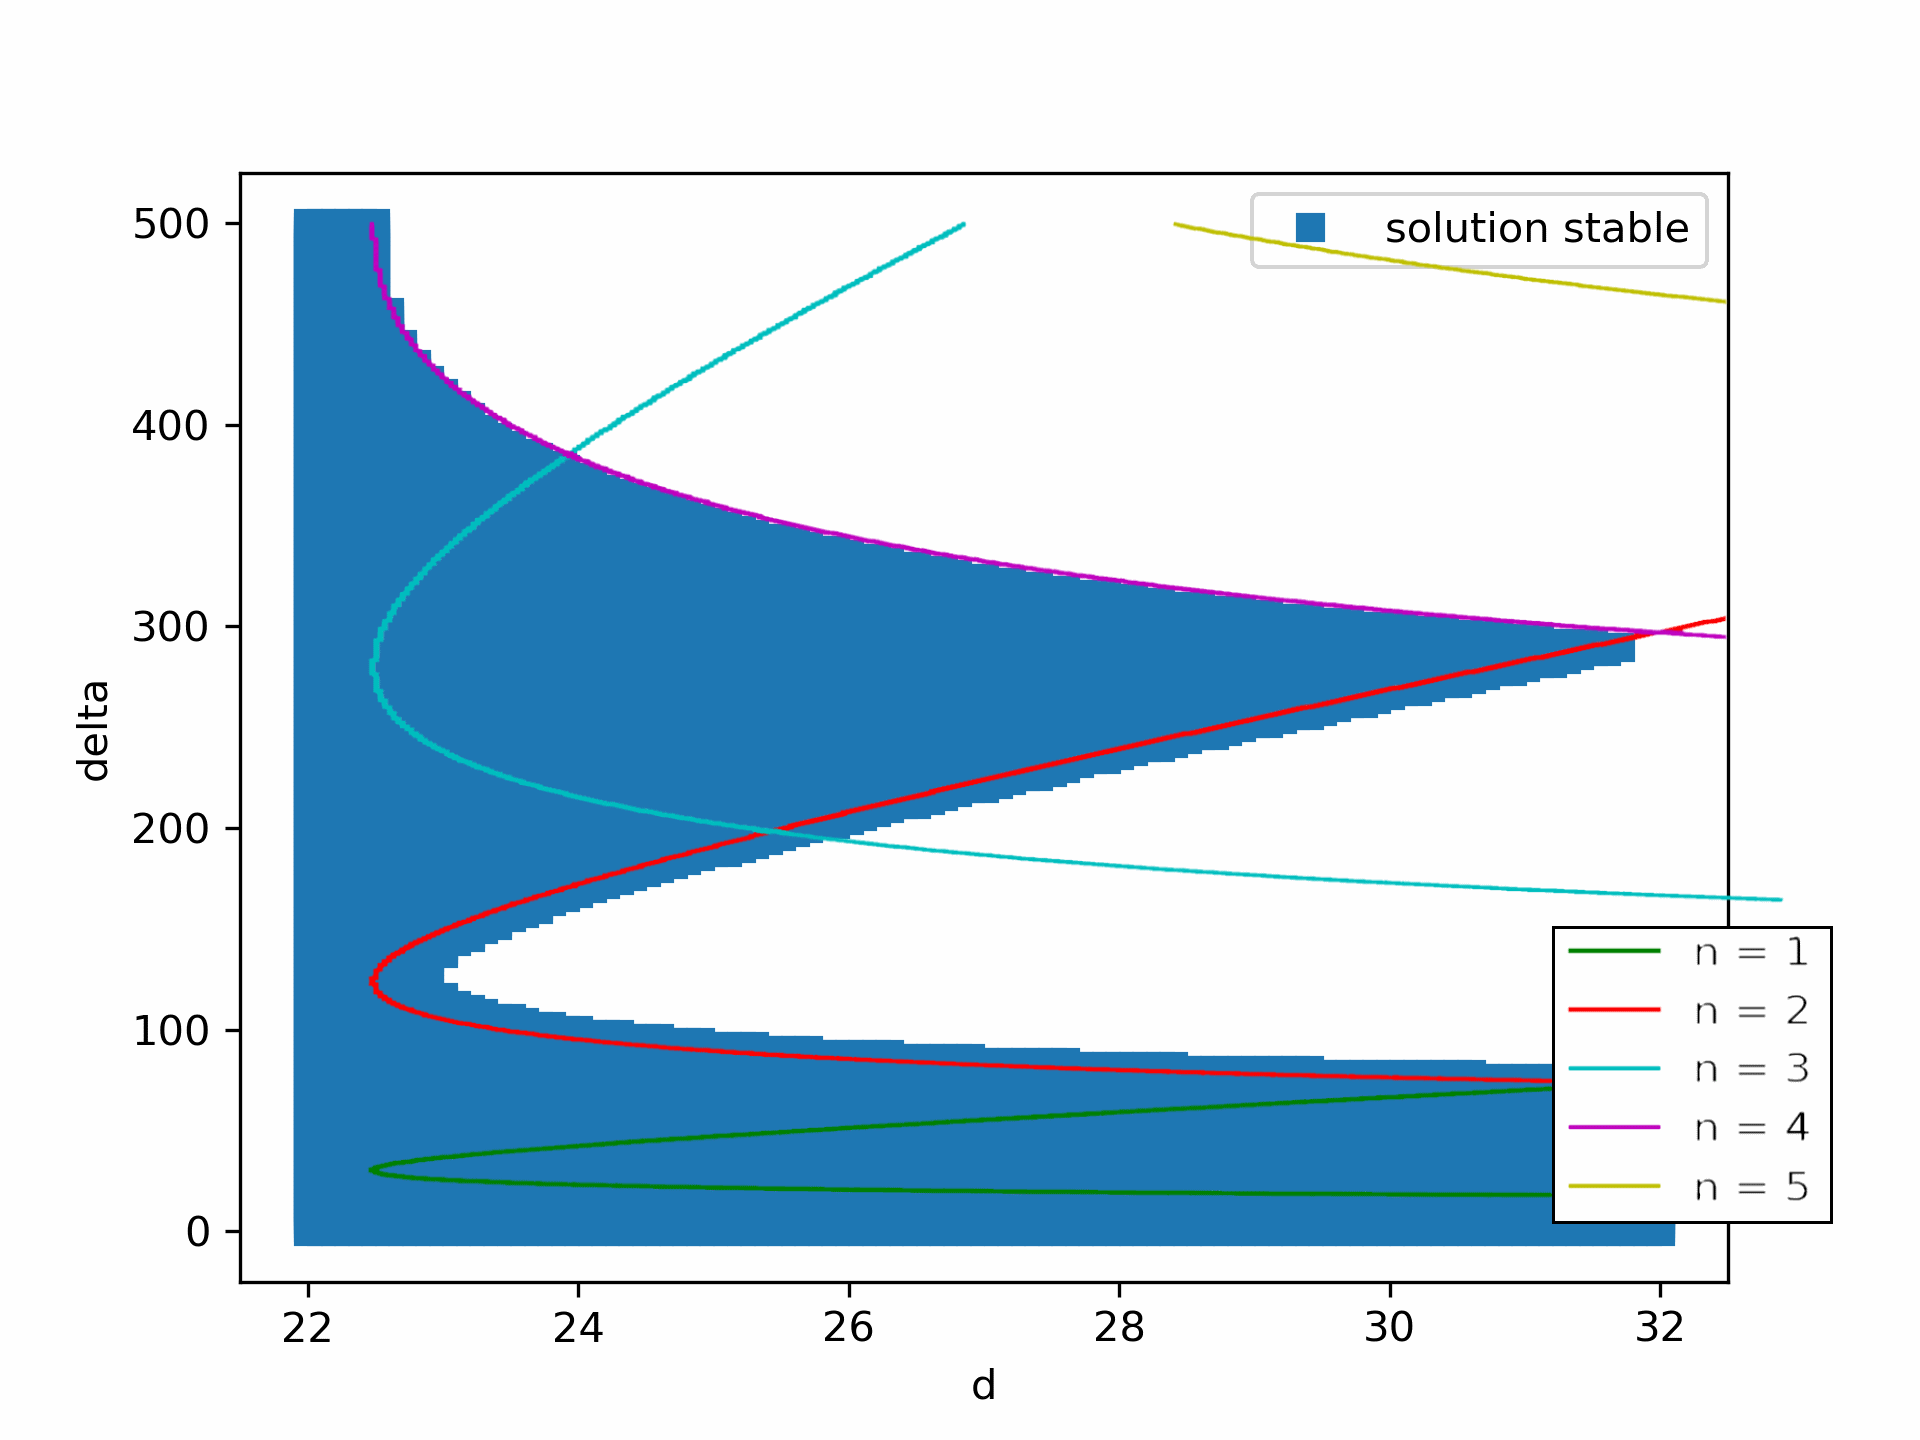
\includegraphics[width=0.65\textwidth]{superposition_diagrammes_turing.png}
\caption{Superposition des deux diagrammes}
\end{figure}
Ils coïncident seulement pour les modes pairs (n=4 et n=2).
\end{frame}





%DEBUT DE LA PARTIE DE CYRIL : L'AMPLITUDE DES MODES INSTABLES

\begin{frame}{\'Etude d'un mode instable}
\textbf{Objectif}\\
Prédire théoriquement l'allure de la sollution lorsque $\delta=$150 et $d=d_c +\epsilon$ (avec $\epsilon<<1$)
\begin{figure}
\begin{subfigure}
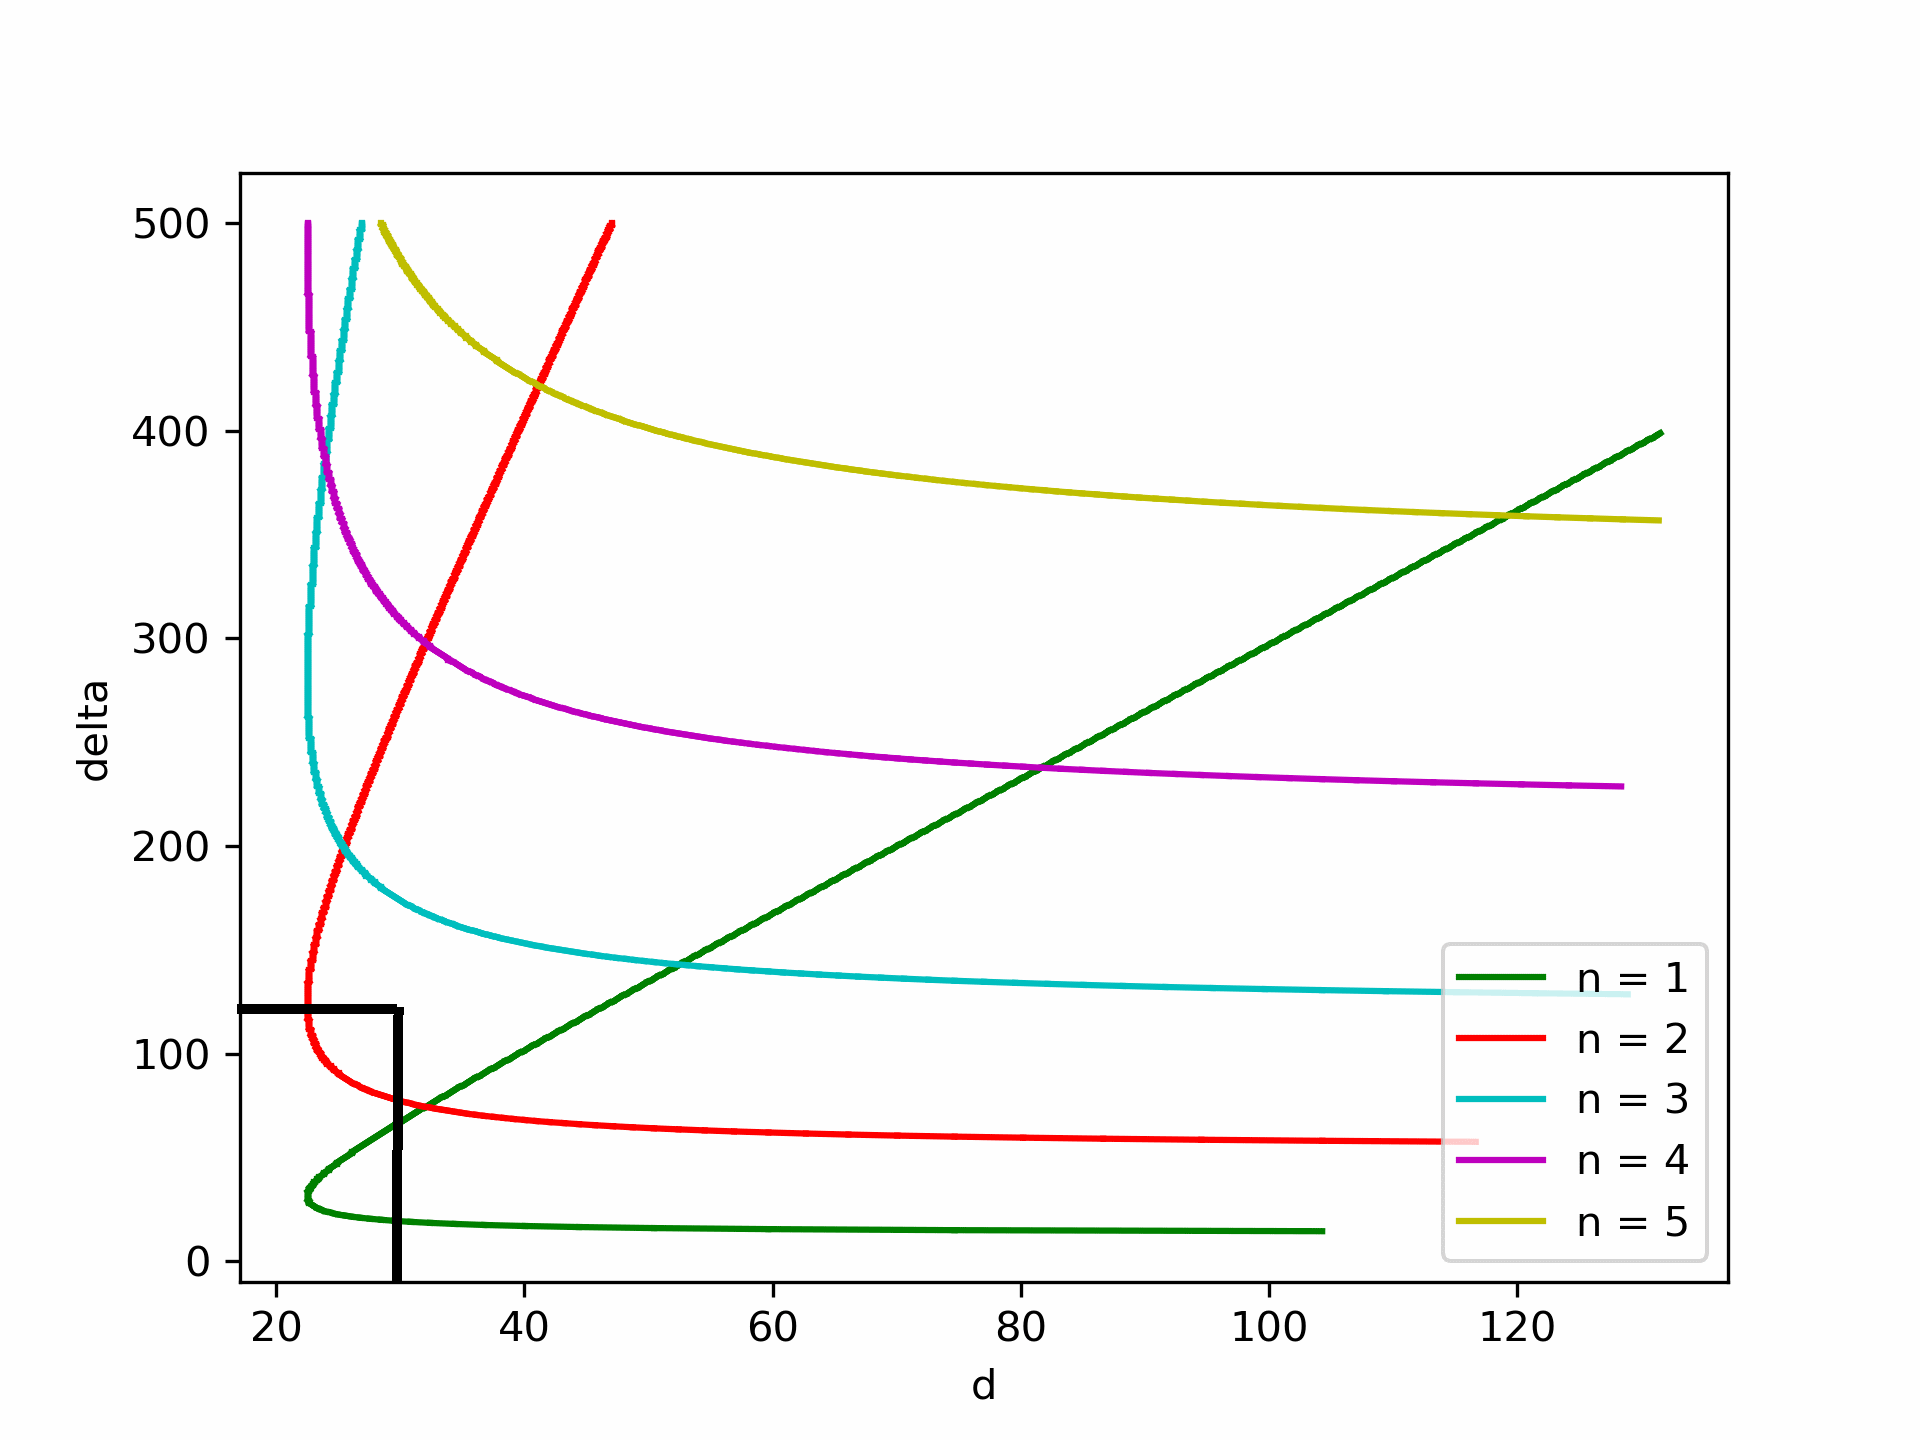
\includegraphics[width=0.4\textwidth]{diagrammes_turing1.png}
\end{subfigure}
\begin{subfigure}
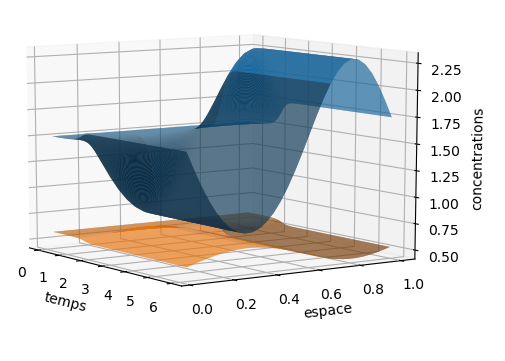
\includegraphics[width=0.4\textwidth]{graph1.png}
\end{subfigure}
\caption{\label{fig:graph1}Instabilité du mode 2}
\end{figure}
\end{frame}

\begin{frame}{\'Etude d'un mode instable}
\textbf{Apparition d'une sinuoïde}\\
Solution en fonction du temps et de l'espace :
\begin{equation}
    \forall \  t\geq 0 ,\ x \in [0,1], \quad  z(x,t) = \sum_{n=0}^{\infty} s_{n}(t)e_{n}(x)
\end{equation}
Donc : 
\begin{equation}
\begin{split}
    \forall n \in \mathbb{N}, \quad \frac{d s_{n}}{dt} & = -(n \pi)^{2}D s_{n} + \delta J_{f}(c_{eq}) s_{n} \\
    & = B_{n} s_{n}
\end{split}
\end{equation}
Or pour le choix de $\delta$ et $d$, $s_n \longrightarrow 0$ sauf pour $n=2$ (et $n=0$) car $det(B_2)<0$ ! Cela explique en partie la forme de la solution.
\end{frame}

\begin{frame}{\'Etude d'un mode instable}
\textbf{Résolution directe}\\
Méthode issue de l'article sur la formation des patterns écrit par Antoine Levitt : on développe la solution en série paramètrée par $\xi$
\begin{equation}
c(x) = \sum_{n=0}^{\infty} \epsilon^{\xi n} c_n (x)
\end{equation}
On injecte dans l'équation : 
\begin{equation}
Dc''(x) + f(c)=0
\end{equation}
\end{frame}

\begin{frame}{\'Etude d'un mode instable}
\textbf{Résolution directe}\\
On rassemble les ordre ensemble (en définissant l'opérateur L): 
\begin{equation}
\left\{
    \begin{array}{ll}
        \begin{pmatrix}
        1 & 0\\
        0 & d_c
        \end{pmatrix} c_0'' + f(c_0) = 0\ \   pour\ ordre\ 0
        \\
        \\
        \begin{pmatrix}
        1 & 0\\
        0 & d_c
        \end{pmatrix} c_1'' + df(c_0)c_1=Lc_1=0\ \   pour\ ordre\ en\ \xi
    \end{array}
\right.
\end{equation}
On trouve alors :
\begin{equation}
\left\{
    \begin{array}{ll}
        c_0 = \begin{pmatrix} u_{eq} \\ v_{eq} \end{pmatrix}
        \\
        \\
        c_1(x) = A cos(jx)e_2
    \end{array}
\right.
\end{equation}
où $e_2$ est tel que $Vect(e_2)=Ker(B_2)$. Cette forme correspond assez bien à l'étude qualitative. 
\end{frame}

\begin{frame}{\'Etude d'un mode instable}
\textbf{Résolution directe}\\
À cause du terme $d_c + \epsilon$ dans la matrice de diffusion, un terme porté par $\epsilon^{\xi +1}$ apparait : 
\begin{equation}
\epsilon^{\xi +1} v_1 ''   \begin{pmatrix}
        1 \\
        0 
        \end{pmatrix} 
\end{equation}
Cet ordre ne peut pas être isolé sinon $v_1 ''=0$ ce qui est incompatible avec la forme trouvée de $c_1$. La seule possibilité est que : 
\begin{equation}
    \xi+1=n\xi
\end{equation}
\end{frame}

\begin{frame}{\'Etude d'un mode instable}
\textbf{Résolution directe}\\
Lemme : Alternative de Fredholm\\
Si L est un opérateur linéaire borné sur $L_2([0,1],\mathbf{R} ^2)$ et $f$ une fonction, une condition d'existence d'une fonction $w$ tel que $Lw=f$ est que $f\in Ker(L)$
\newline 
\newline En étudiant la possibilité que n=3 i.e on rassemble les termes en $\epsilon^{3\xi}$, on remarque grâce à l'alternative de Fredholm que c'est la seule possibilité. Ainsi :
\begin{equation}
    \xi=\frac{1}{2}
\end{equation}
\textbf{Solution approchée}
\begin{equation}
c(x)\simeq\overline{c} + A \sqrt{\epsilon} cos(jx)e_2
\end{equation}
\textbf{Remarque}\\
Le résultat ci-dessus est assez satisfaisant étant donné l'allure de la solution numérique.
\end{frame}

\begin{frame}{\'Etude d'un mode instable}
\textbf{Tests numérique}\\
\begin{figure}
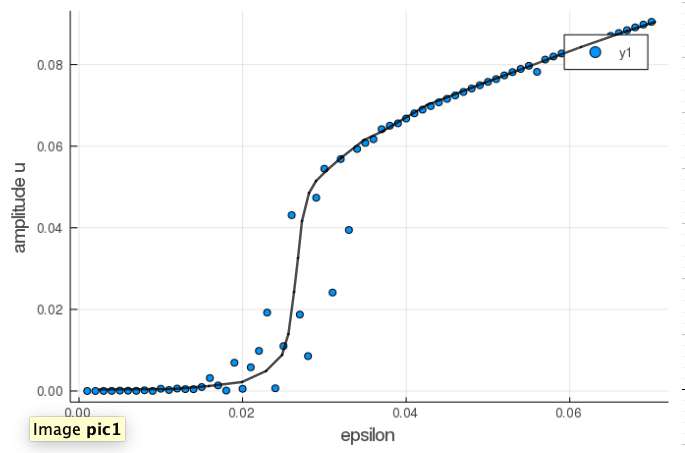
\includegraphics[width=0.7\textwidth]{ampli.png}
\caption{\label{fig:graph4} pseudo-amplitude en fonction de $\epsilon$ et courbe de tendance}
\end{figure}
Les points sont plus dispersés autour du point d'inflexion en raison de la remarque faite plus tôt i.e 
\end{frame}

\begin{frame}{\'Etude d'un mode instable}
\textbf{Remarques sur la simulation}\\
\begin{itemize}
    \item La courbe est volontairement décalée pour pouvoir constater le changement de comportement asymptotique lorsqu'on franchit $d_c$. On peut d'ailleurs donner une valeur plus précise de $d_c$ à l'aide de ce test : $d_c\simeq 22,47$
    \item Les points sont plus dispersés autour du point d'inflexion en raison de la remarque faite plus tôt i.e plus on s'approche de $d_c$, plus la convergence est tardive. Ainsi il aurait fallu des temps très longs et la machine le supportait mal.
    \item La tendance n'est pas exactement une fonction racine, mais proche de $d_c$ on remarque quand même une pente qui semble bien redressée. Cette caractéristique va tout de même dans le sens de l'approximation de $c$ trouvée.
\end{itemize}
\end{frame}

%FIN DE LA PARTIE DE CYRIL

\end{document}
